\question Find a cubic (3-regular) graph without a perfect matching.

\begin{solution}
  Consider the following graph. We claim that this has no perfect matching. 

  \begin{center}
    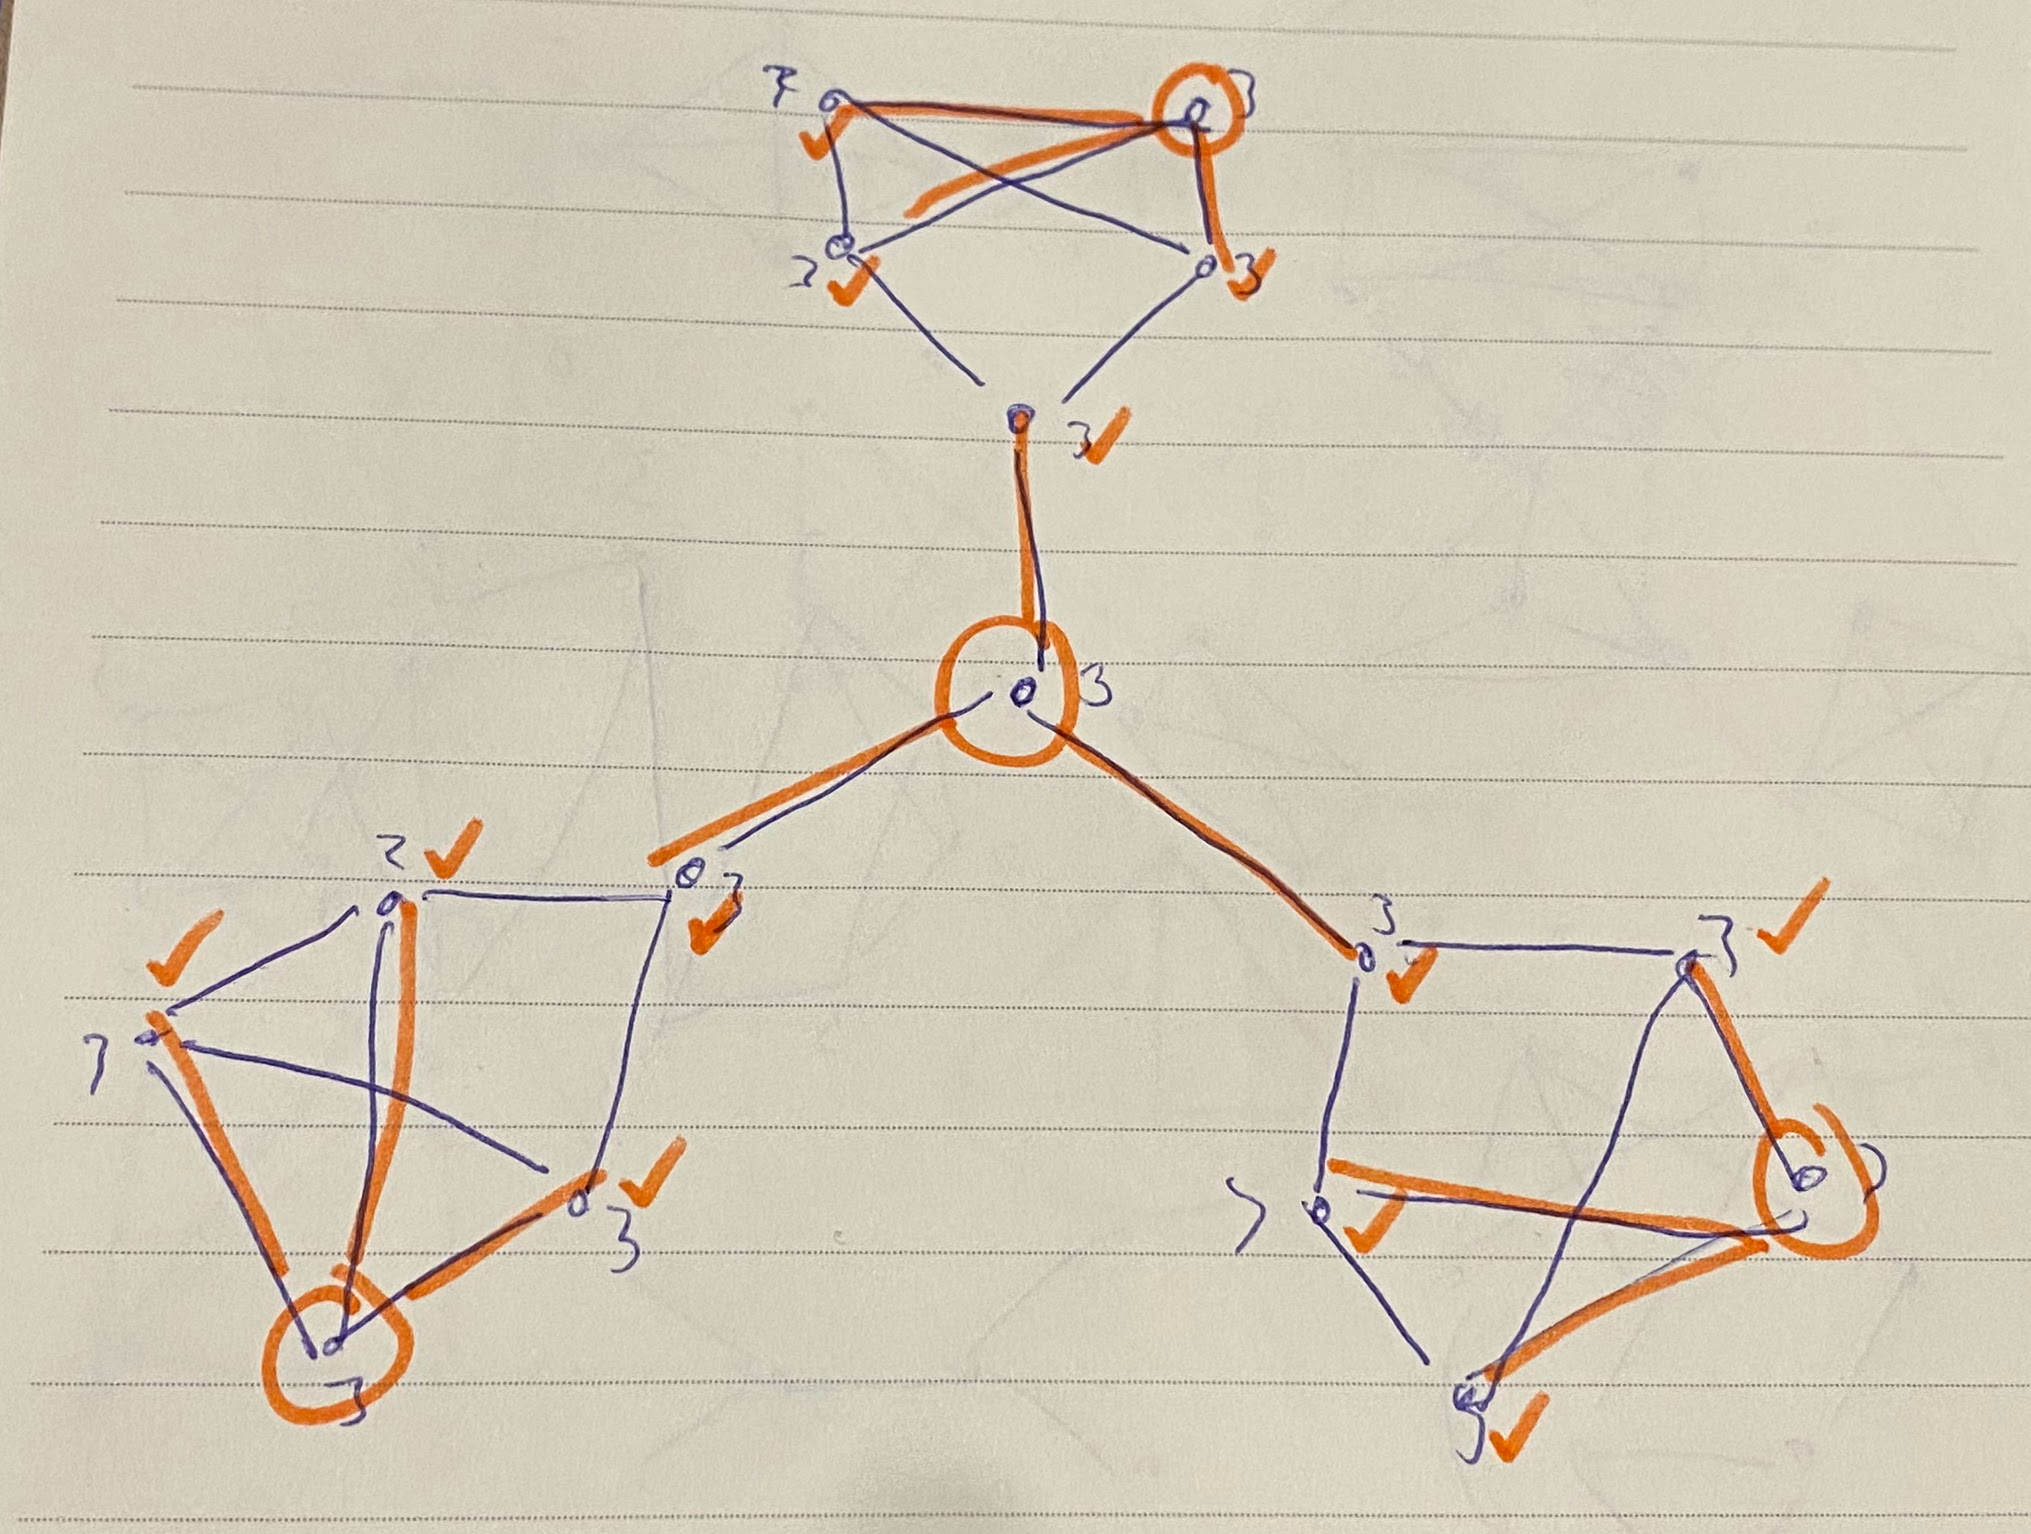
\includegraphics[width=0.69\textwidth]{figures/p2-soln}
  \end{center}

  While we may be unable to show that this vertex cover (circled) is minimal, we
  can see that we can use 4 vertices to make a vertex cover of this graph. Thus,
  by K\"onig's Theorem, the maximum number of matching in this graph cannot be
  greater than 4. Since this graph contains 16 vertices, a matching of size 4
  only contains 8 vertices. Therefore, there is no perfect matching on this graph.
\end{solution}
